\chapter{My contribution}
\label{cha:MyContribution}

This chapter focuses on the implementation of a new segmentation approach by taking the existing methods as reference (see chapter \ref{cha:relatedWork}). 

\section{Goal and approach}

The goal is to segment an articulated mesh $M$ into its unknown number $n$ of rigid parts $ P =  \{ {p_0,....p_n}\}$ and extract the joints $ J =  \{ {j_0,....j_{n-1}}\}$ linking those parts in form of a skeleton structure. In general, this is done by non-rigid registration of the points clouds $S\textsubscript{0}$ and $D\textsubscript{0}$ of an object in two different poses. $S_0$ is thereby used as a \textit{template} to be registered with $D_0$. The main task is to determine a part assignment $p_i$ and the corresponding transformation $t_i$ for all points of the \textit{template} that alligns them with all points of $D_0$. Basically, a divide and conquer approach (see section \ref{divideAndConquer}) is implemented to recursively subdivide $S_0$ and $D_0$ into clusters trying to be matched(reduce the computation steps of the correlated correspondence algorithm \cite{Anguelov04}). Furthermore, the LRP approach \cite{correspondence} is employed as an initial registration step to align the two poses of the object. 

\section{Assumptions}

The input mesh $M$ is assumed to solely consist of rigid parts that can not be deformed or stretched (e.g. rigid parts of a human). Those parts are linked by joints and no matter what kind of pose is adopted by the articulated object, the geodesic distances bestween mesh points always stay the same (see Figure SKIZZE).  Thereby, it is taken advantage of the knowledge that points located on a rigid part $p_i$ have the same transformation $t_i$ . Furthermore, it is assumed that the two poses $S_0$ and $D_0$ of $M$ are oriented the same direction.

\section{Challenges/restrictions}

There are many challenges regarding the non-rigid registration of point clouds in 2D, as well as in 3D. First off, the input data can be noisy by means of points not belonging to the object. Furthermore, the approach is computationally expensive and time-consuming, as the corresponding body parts of two meshes need to be detected iteratively. Additionally, the inevitable difficulty of finding the global optimum, related to ambiguous body parts, has to be overcome.

\section{Approach}
\label{divideAndConquer}

\subsection{Divide and conquer}

 The algorithm starts with two sets of point clouds $S_0$ and $D_0$ of an object $M$ in different poses (\ref{fig:dc_original_p2}). The two point clouds are iteratively subdivided into point clusters $ C =  \{ {c_0,..., c_m}\}$ through their centroids. In each iteration step two related clusters of $S_0$ and $D_0$ are matched by applying the ICP (iterative closest point) resulting in a matching error $e$. In case of $ e < \tau $, two clusters are assumed to match. Otherwise, the algorithm is applied recursively and the clusters are again subdivided into further clusters. The algorithm terminates if all resulting clusters of $S_0$ can be matched to all clusters of $D_0$. All neighboring clusters are then checked to be merged, in case of having divided a rigid part. After that step the remaining clusters are assigned to a rigid part $part_i$. 
 
 \subsection{Removing outliers}
 
 As a first step the outliers of the two point clouds S0 and D0 are removed. This is done, by finding clusters and just keeping the biggest one, assuming it is the main object
 
 \subsection{Subdividing into clusters}
 
 As a next step, the two point clouds $S_0$ and $D_0$ are assigned to the initial clusters $c_0$. If the matching between them does not suceed, they are subdivided into two clusters and the whole procedure is repeated recursively until all sub clusters $C = \{{c_1, ... c_m}\} $of $S_0$ can be matched to the clusters of $D_0$.  $S_0$ and $D_0$ are initially divided into a left and right cluster. 
 
 \subsubsection{Divider position}
 
 To determine where to divide a cluster into two other clusters, PCA is applied on the clusters is applied. The resulting dividers $d_0$ are realised by computing the principal axes $p_0$ through the centroids $ct_0$ and taking the perpendicular secondary axes $s_S$ and $s_D$ through the centroids.
 
 \subsubsection{Cluster tree}
 \label{tree}
 
 The subdividing of the clusters $c_0$ is realised by a depth-first approach in a binary tree. Consequently, $S_0$ and $D_0$ are subdivided from the left to the right. A node $N$ of the tree contains two related clusters $c_i$ of $S_0$ and $D_0$ and in case of subdividing it, a Node \textit{left} and \textit{right}, containing the subdivided clusters $c_{i+1}$ and $c_{i+2}$. If two associated clusters in a Node $n_i$ match, no further subdividing is performed. The resulting leaves of the three are stored as matching clusters $C = \{{c_1, ... c_m}\}$ \ref{fig:illustrationTree}. By applying the depth-first approach, the neighboring clusters in the list are also neighbouring clusters in the object $S_0$ or $D_0$.  As a result, the skeleton structure from an object can be extracted, where parts are connected by joints.
 
 \begin{figure}
 	\centering
 	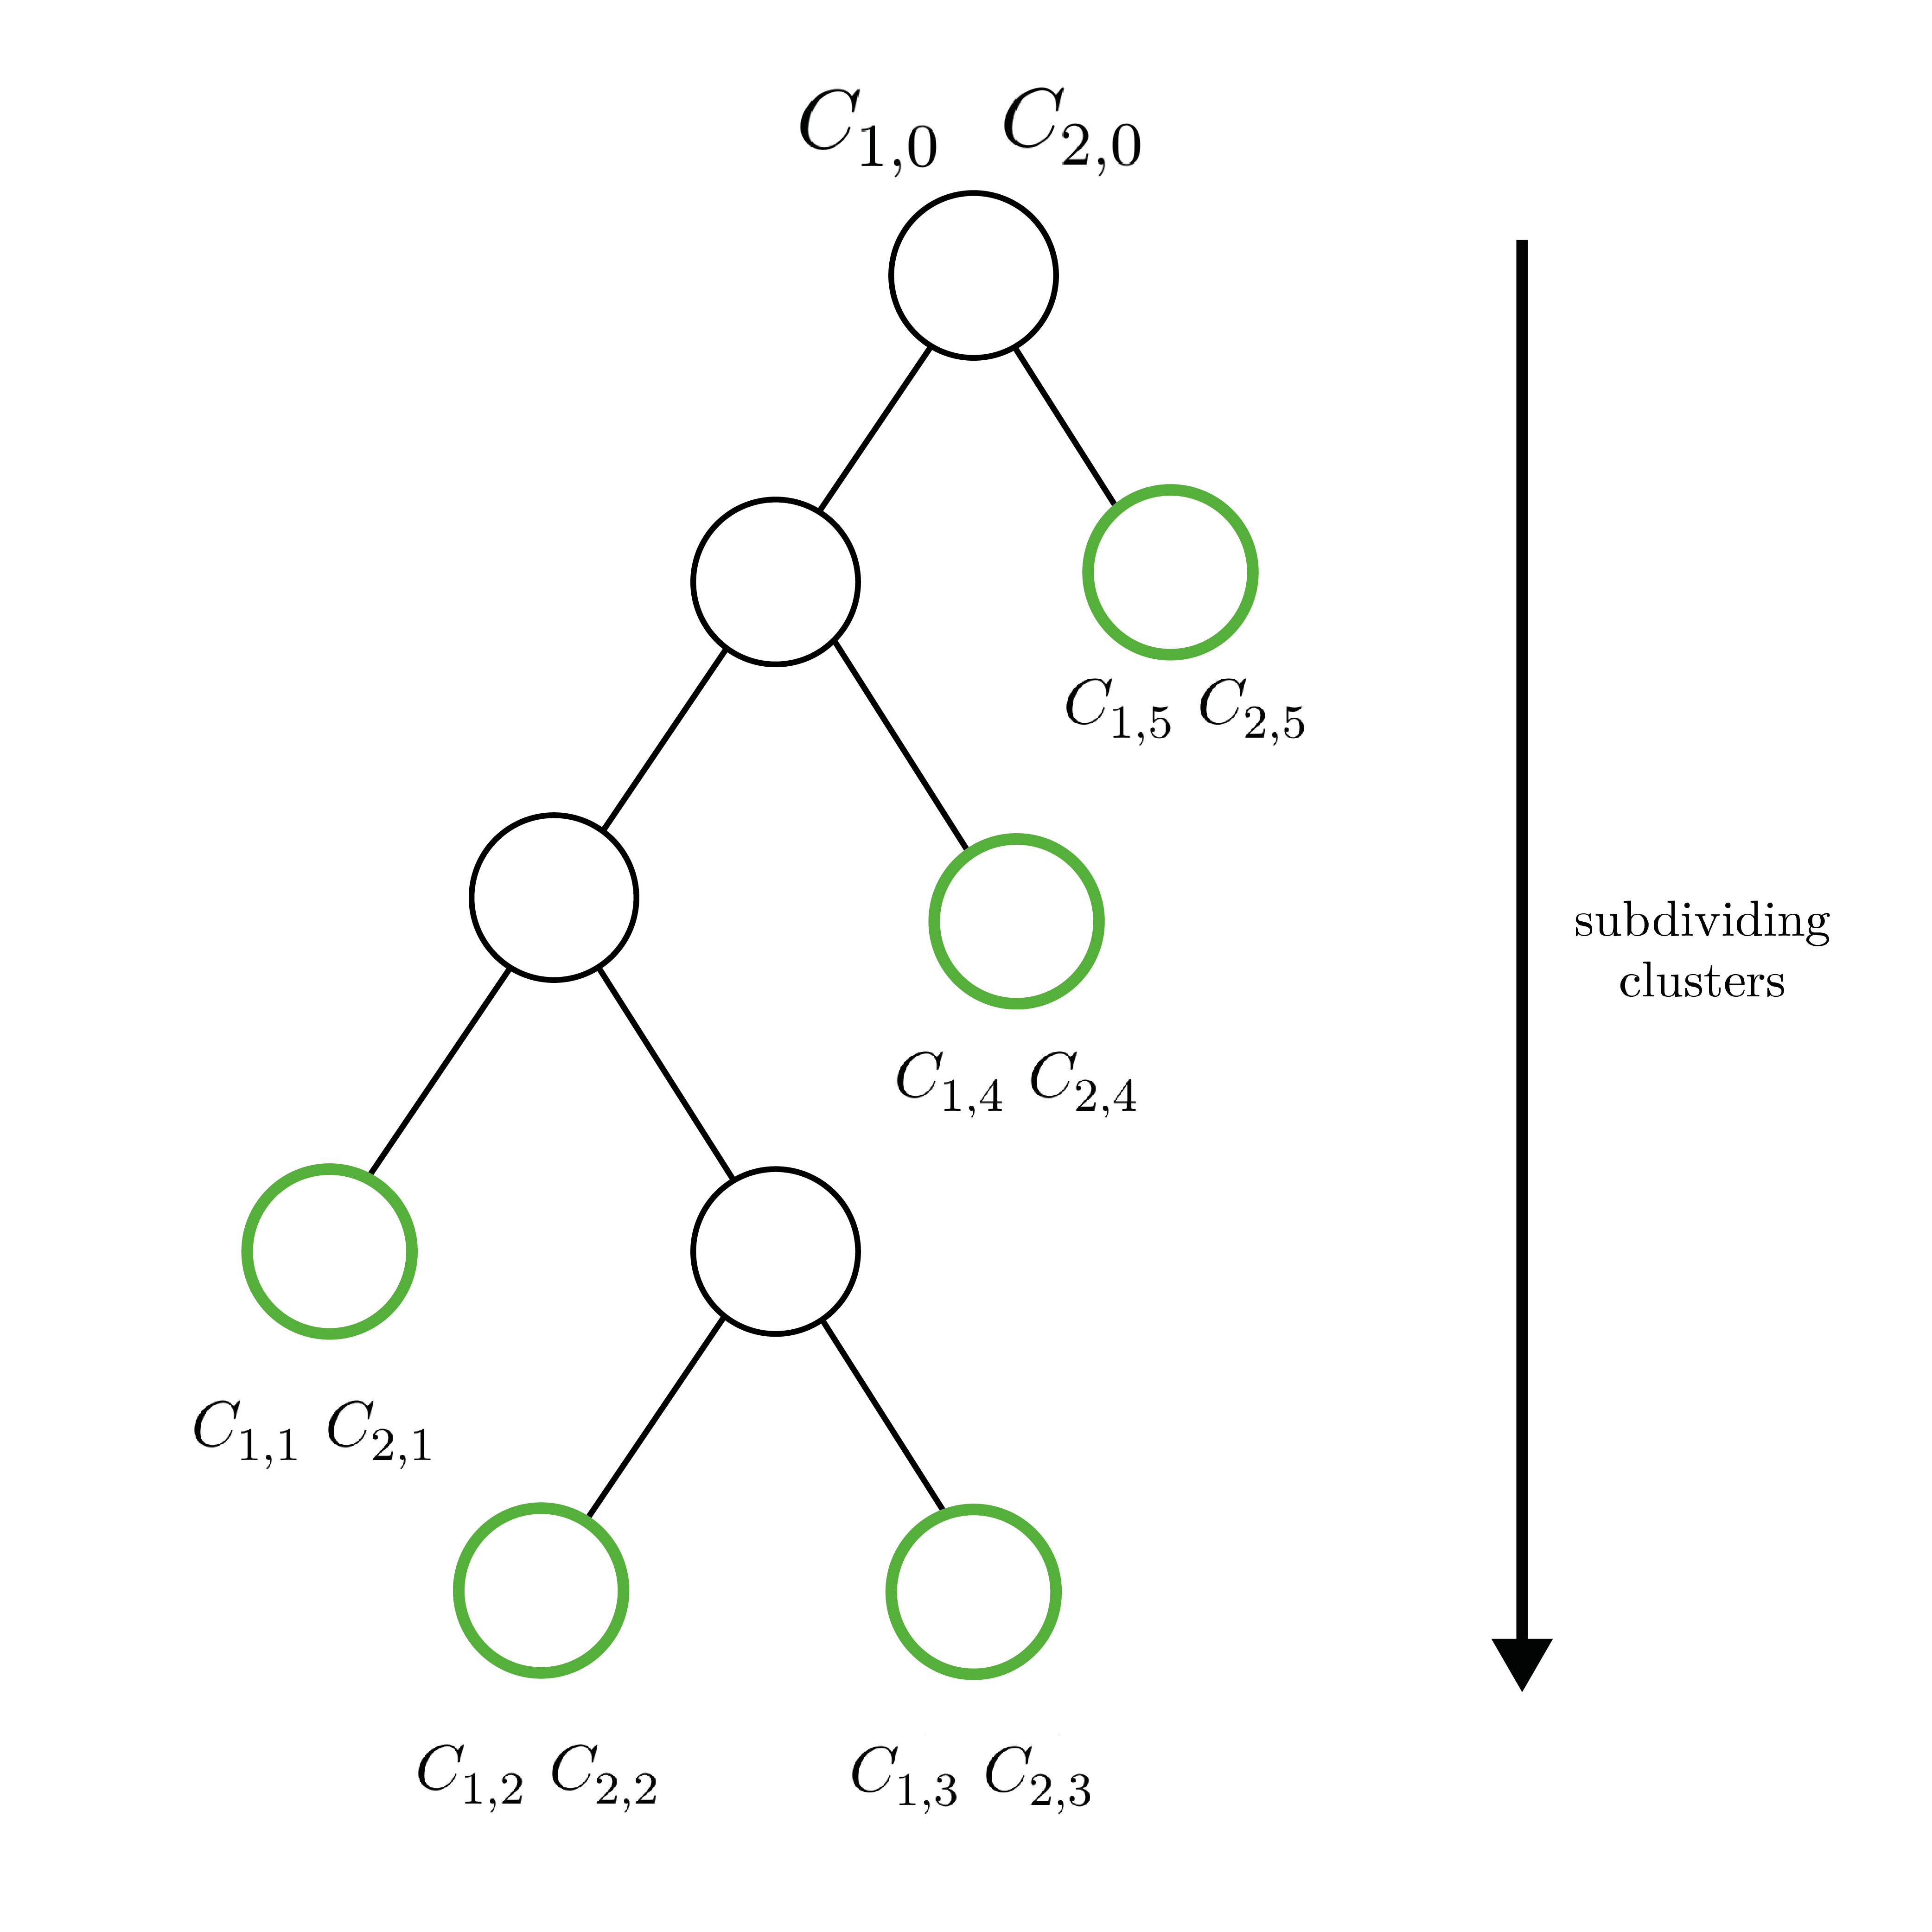
\includegraphics[width=0.7\linewidth]{IllustrationTree}
 	\caption{Subdividing of S0 and D0 into matching clusters by the depth-first approach}
 	\label{fig:illustrationTree}
 \end{figure}
 
 
 \subsubsection{Declaring the matching condition}
 
 By applying the ICP and the nearest neighbour approach, usually a certain matching error is computed between 
 $ P =  \{ {p_0,....p_n}\}$ and its associated points $ Q =  \{ {q_0,....q_n}\}$. To declare when an object is matching, it is important to find the right maximum matching error $\tau$. If it is too high, two clusters are not easy to be matched, which will result in more clusters. If the value is too low, clusters are more likely to be matched and there won't be enough subdividing. The matching threshold is compared to error per point 
 %
 \begin{equation}
 e_{avg} = \frac{\displaystyle\sum_{i=0}^{m}\| p_i - q_i\|^2}{| P |}
 \end{equation}
 %
 
 which is the average error of a point contributing to the total error. By using the average error instead of the total error, region growing is enabled as the matching error is independent of the amount of points.
 
 \subsection{Merging neighboring clusters to rigid parts}
 
 As a next step, neighboring clusters from the matchedList are iteratively merged and checked for another match. This is done to reduce the found clusters to the rigid parts of the object.
 Again, the mergin of one cluster is done until no further merge for neighboring parts can be done. Subsequently, the cluster is assumed to be a rigid part and saved in a new list. The resulting rigid parts in the list are again neighboring (see figure \ref{fig:clusterChain}). 
 
 \begin{figure}
 	\centering
 	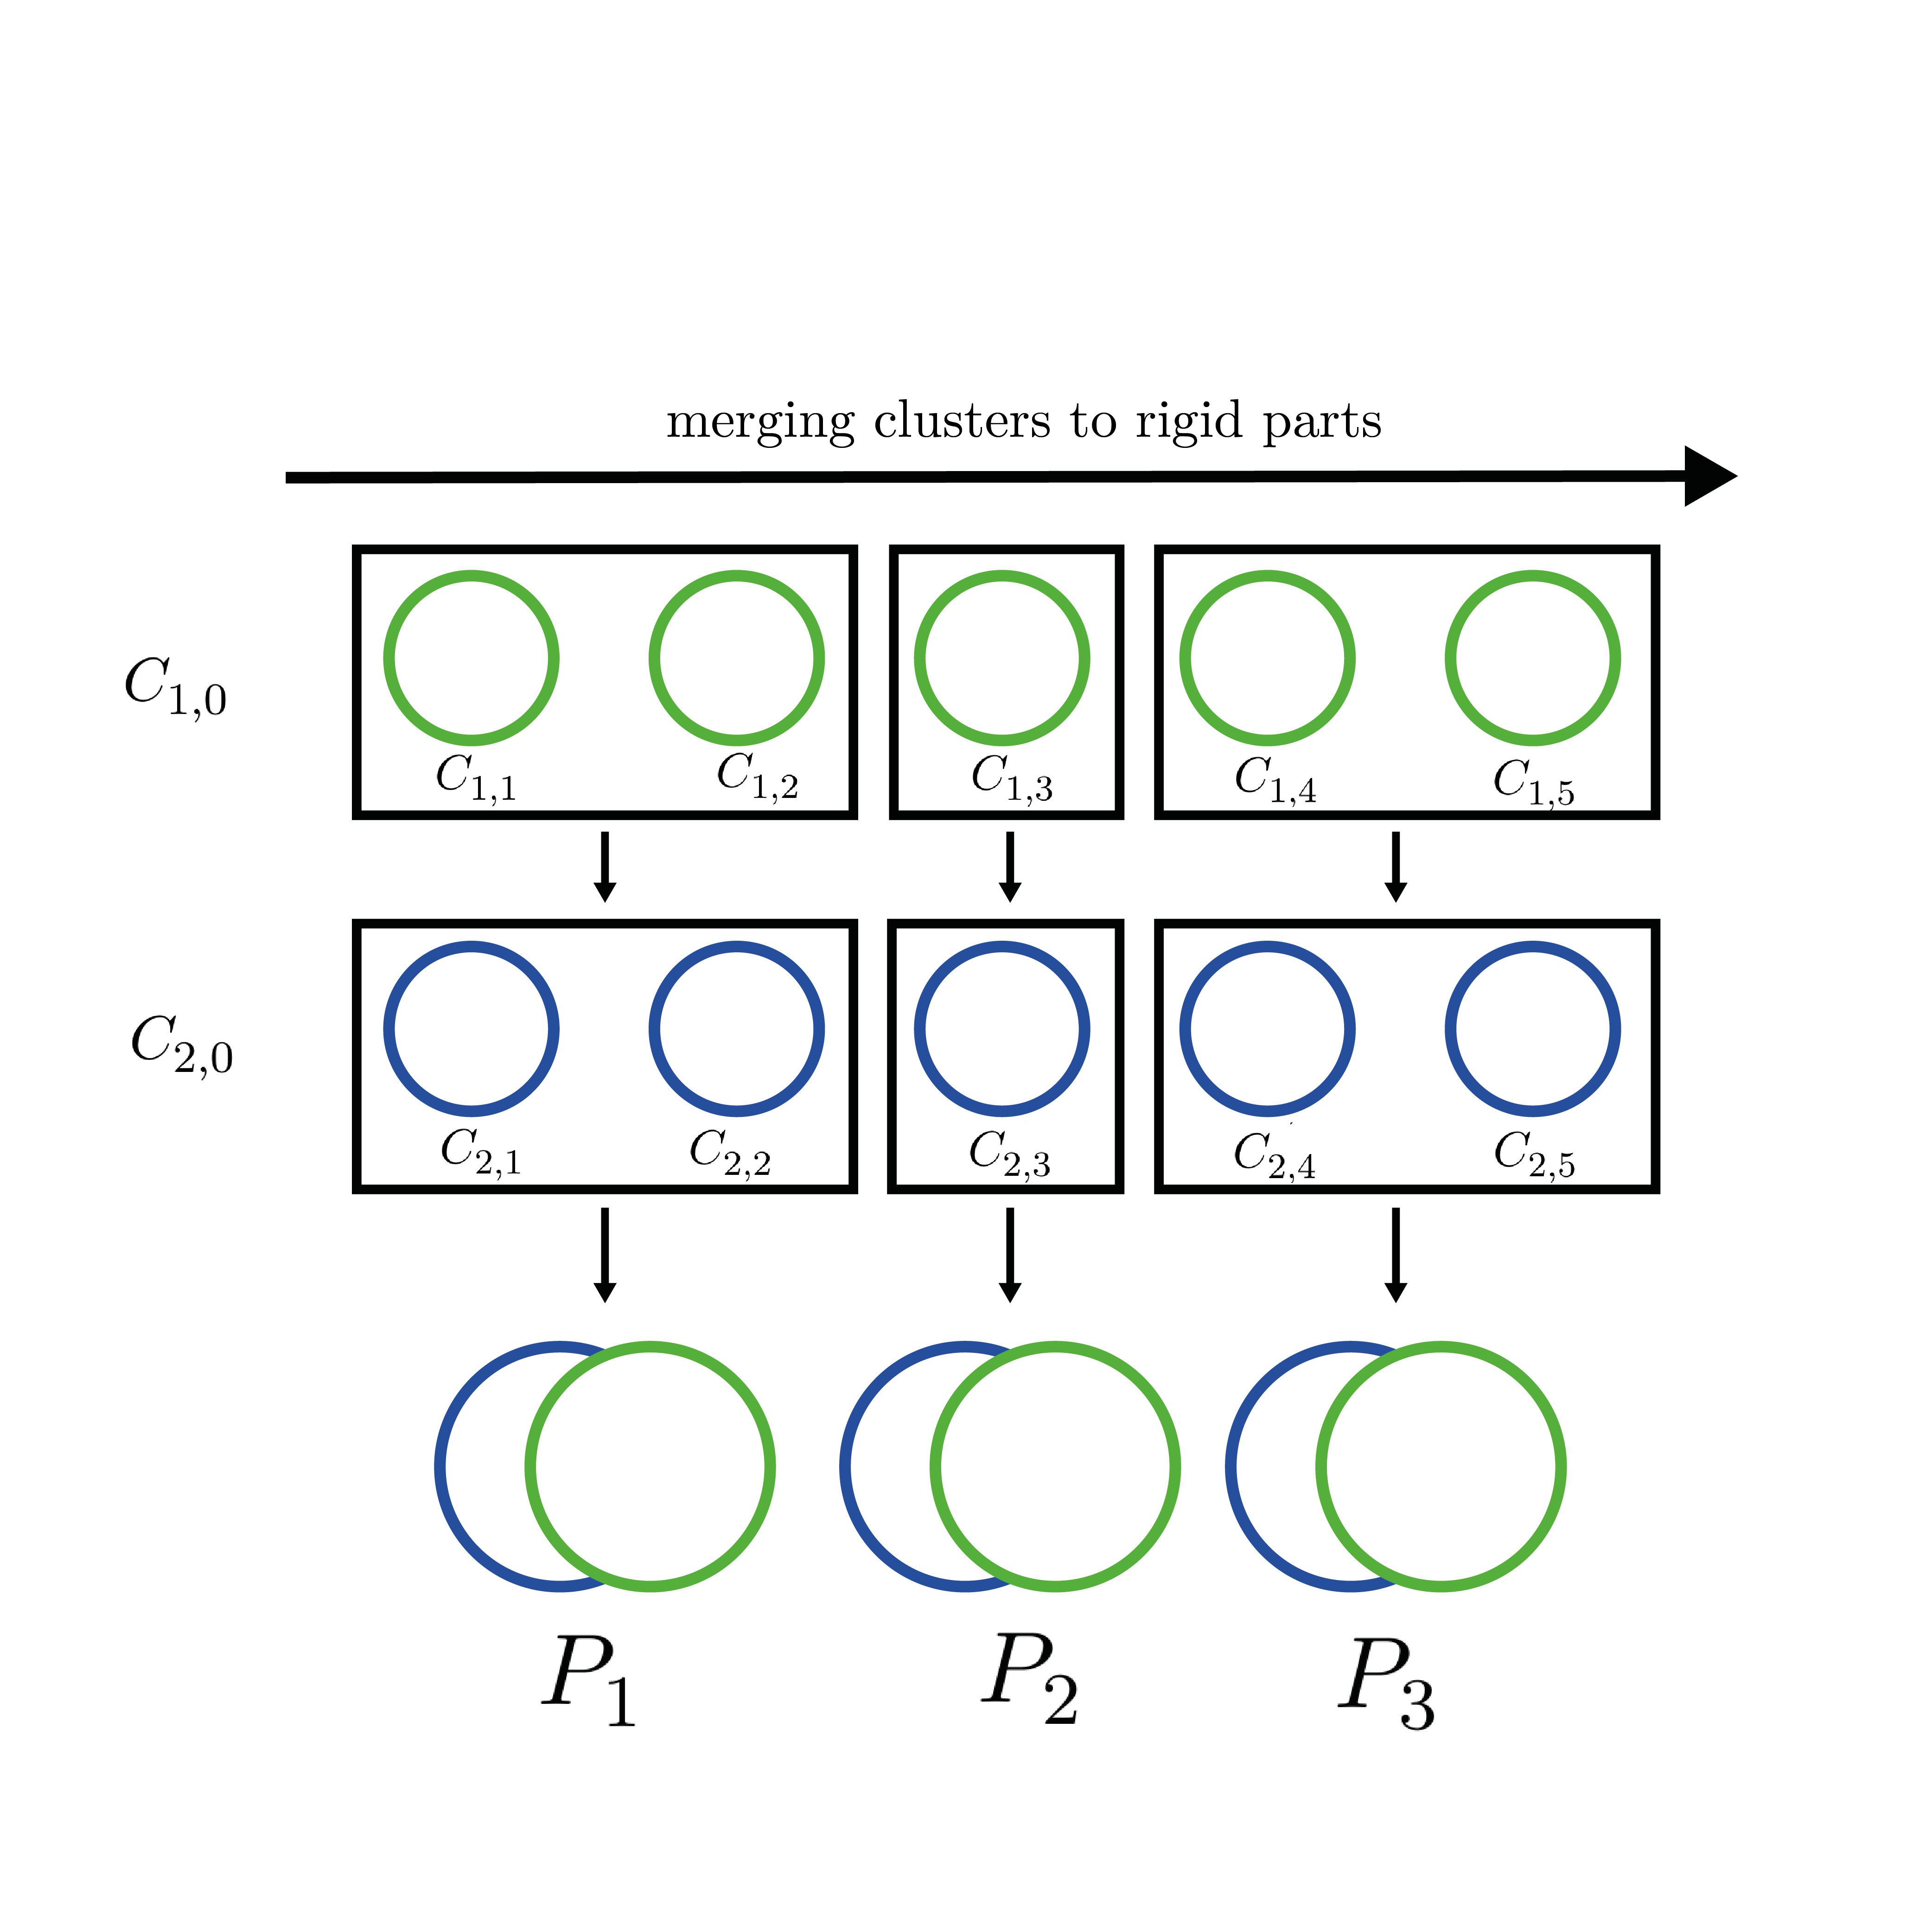
\includegraphics[width=0.7\linewidth]{ClusterChain}
 	\caption{Detecting rigid parts of S0 and D0 by iteratively merging neighboring clusters of S0 and matching them with the merged clusters of DO.}
 	\label{fig:clusterChain}
 \end{figure}
 
 \subsection{Joint/skeleton estimation}
 
 \subsection{Implementation}
 
 using of a binary tree to recursively segment clusters into smaller clusters, until they match. To be continued until all leaves of the tree can be matched with other clusters.
 
  \begin{figure}
  	\centering
  	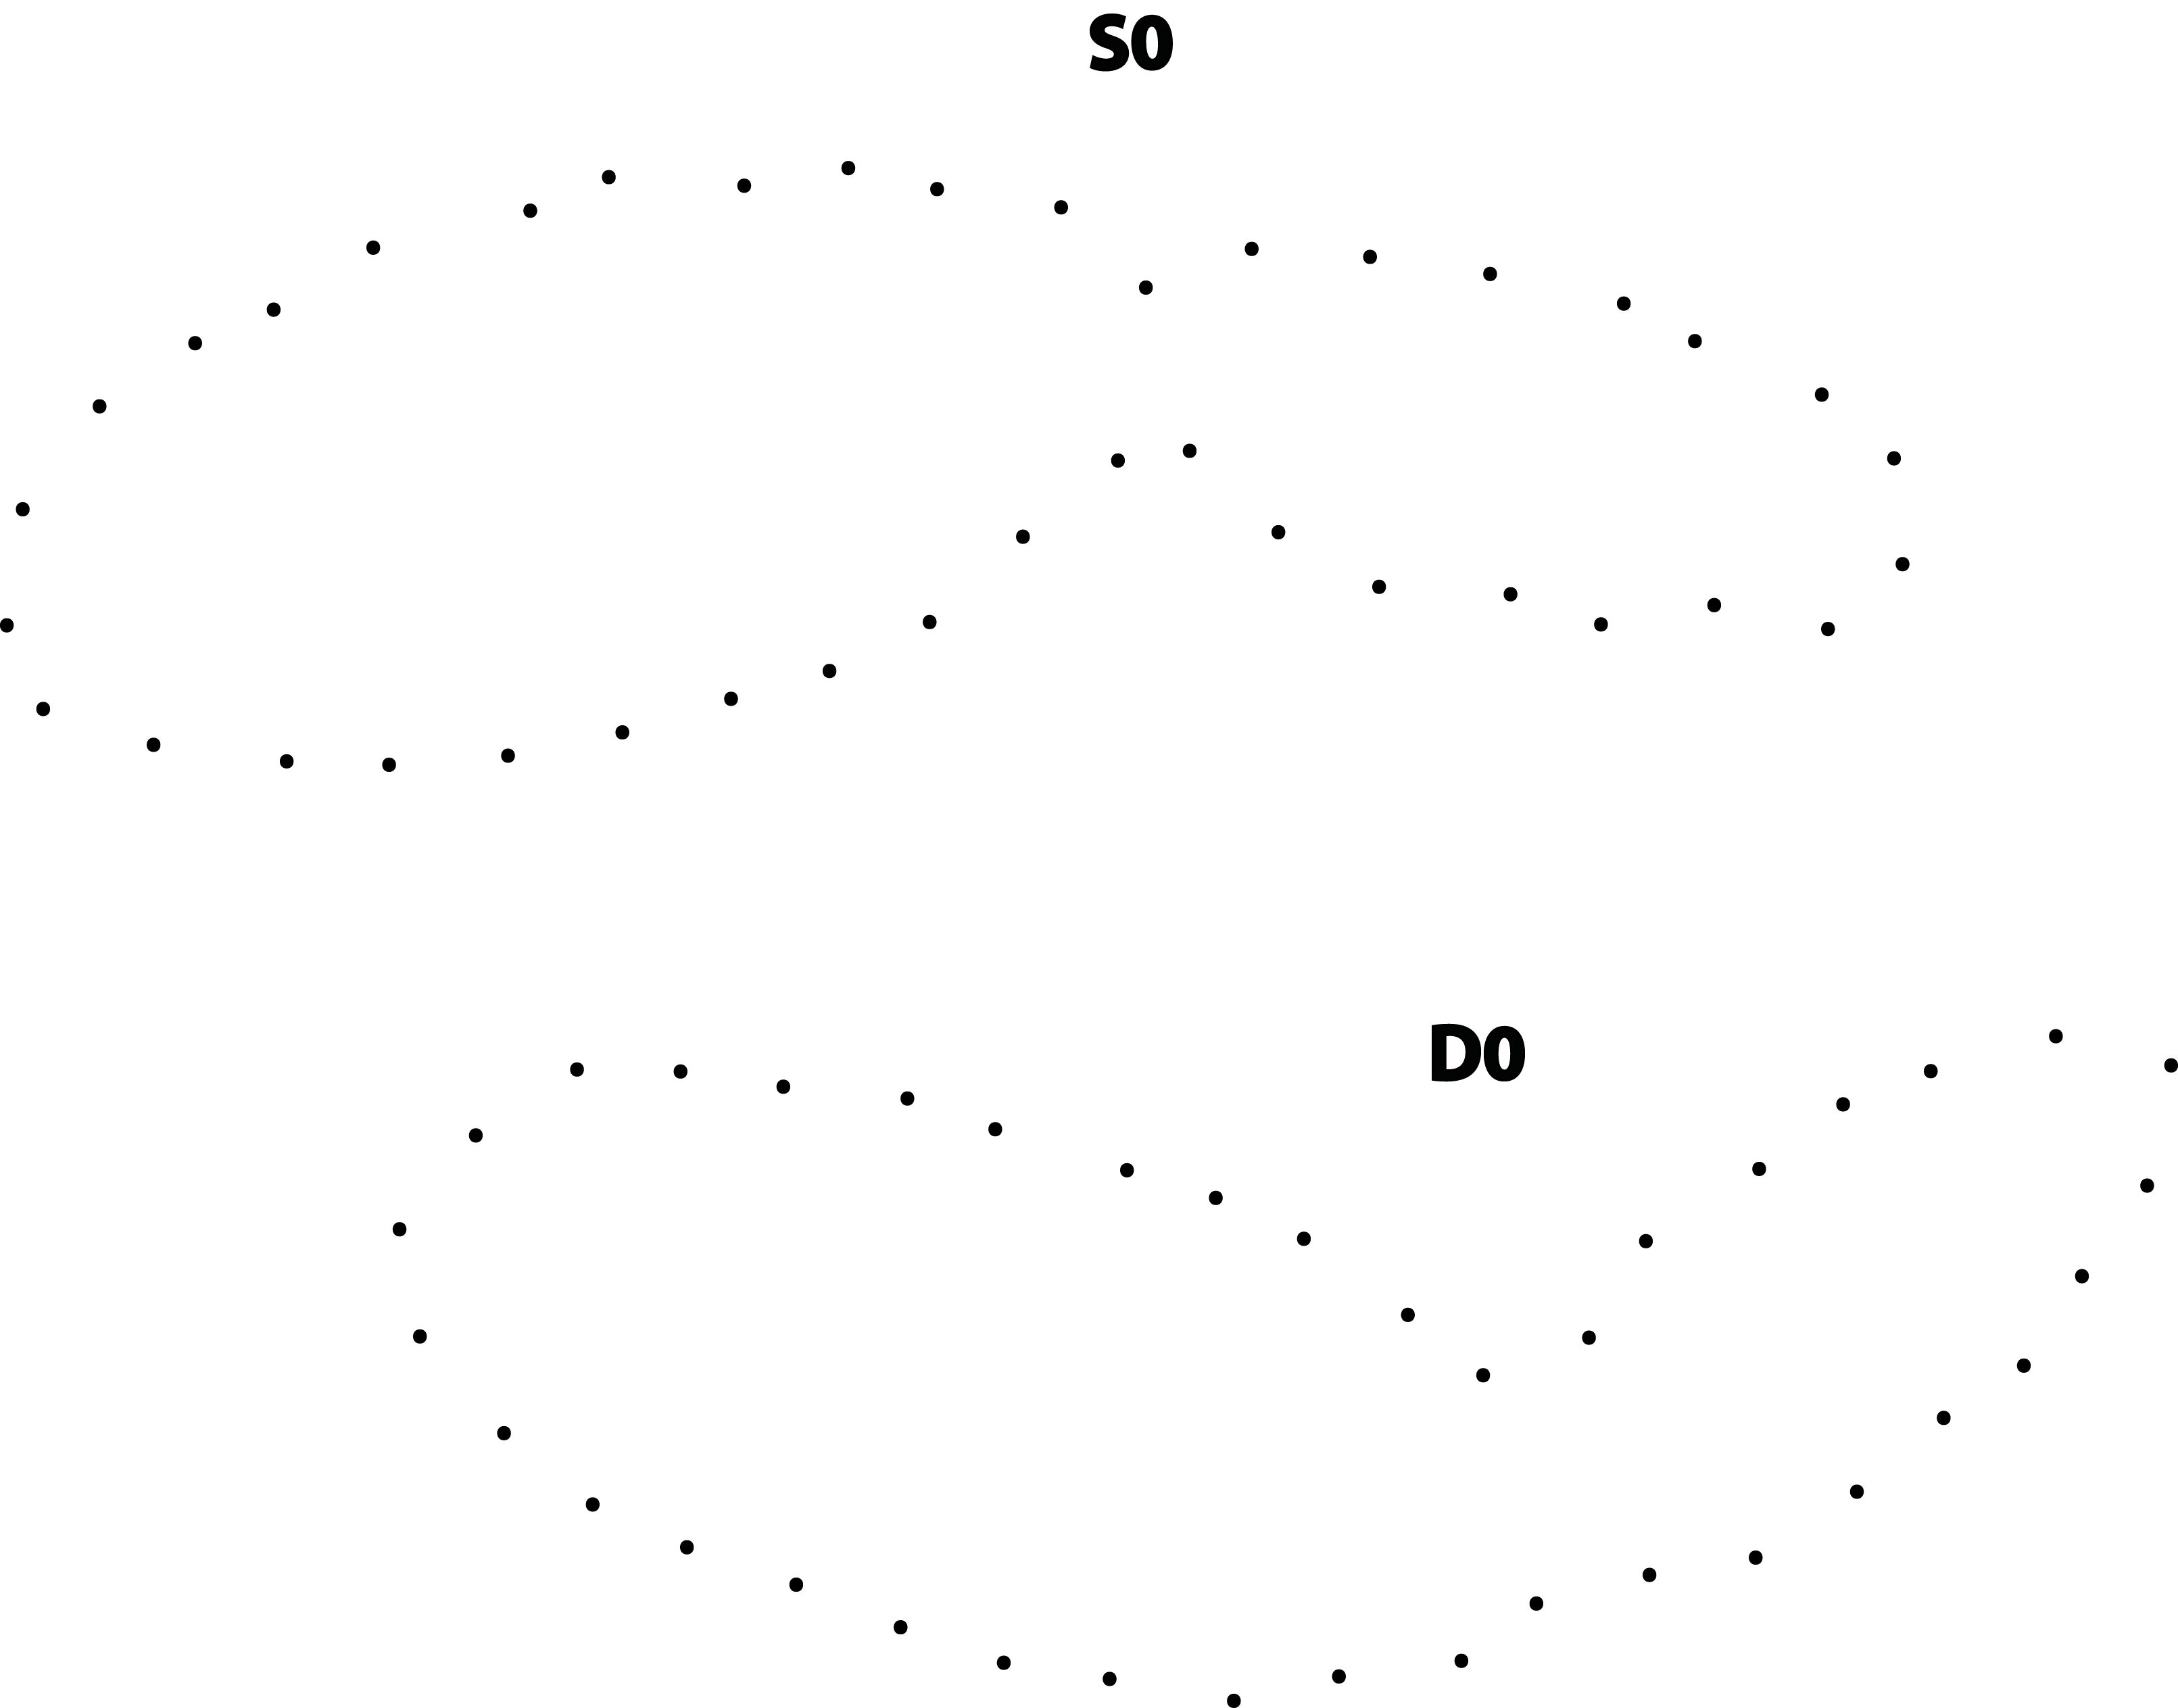
\includegraphics[width=0.7\linewidth]{illustration_original}
  	\caption{Taking a mesh \textit{M} in two different poses \textit{S\textsubscript{0}} and \textit{D\textsubscript{0}} as input.}
  	\label{fig:dc_original_p2}
  \end{figure}
 
 \begin{figure}
 	\centering
 	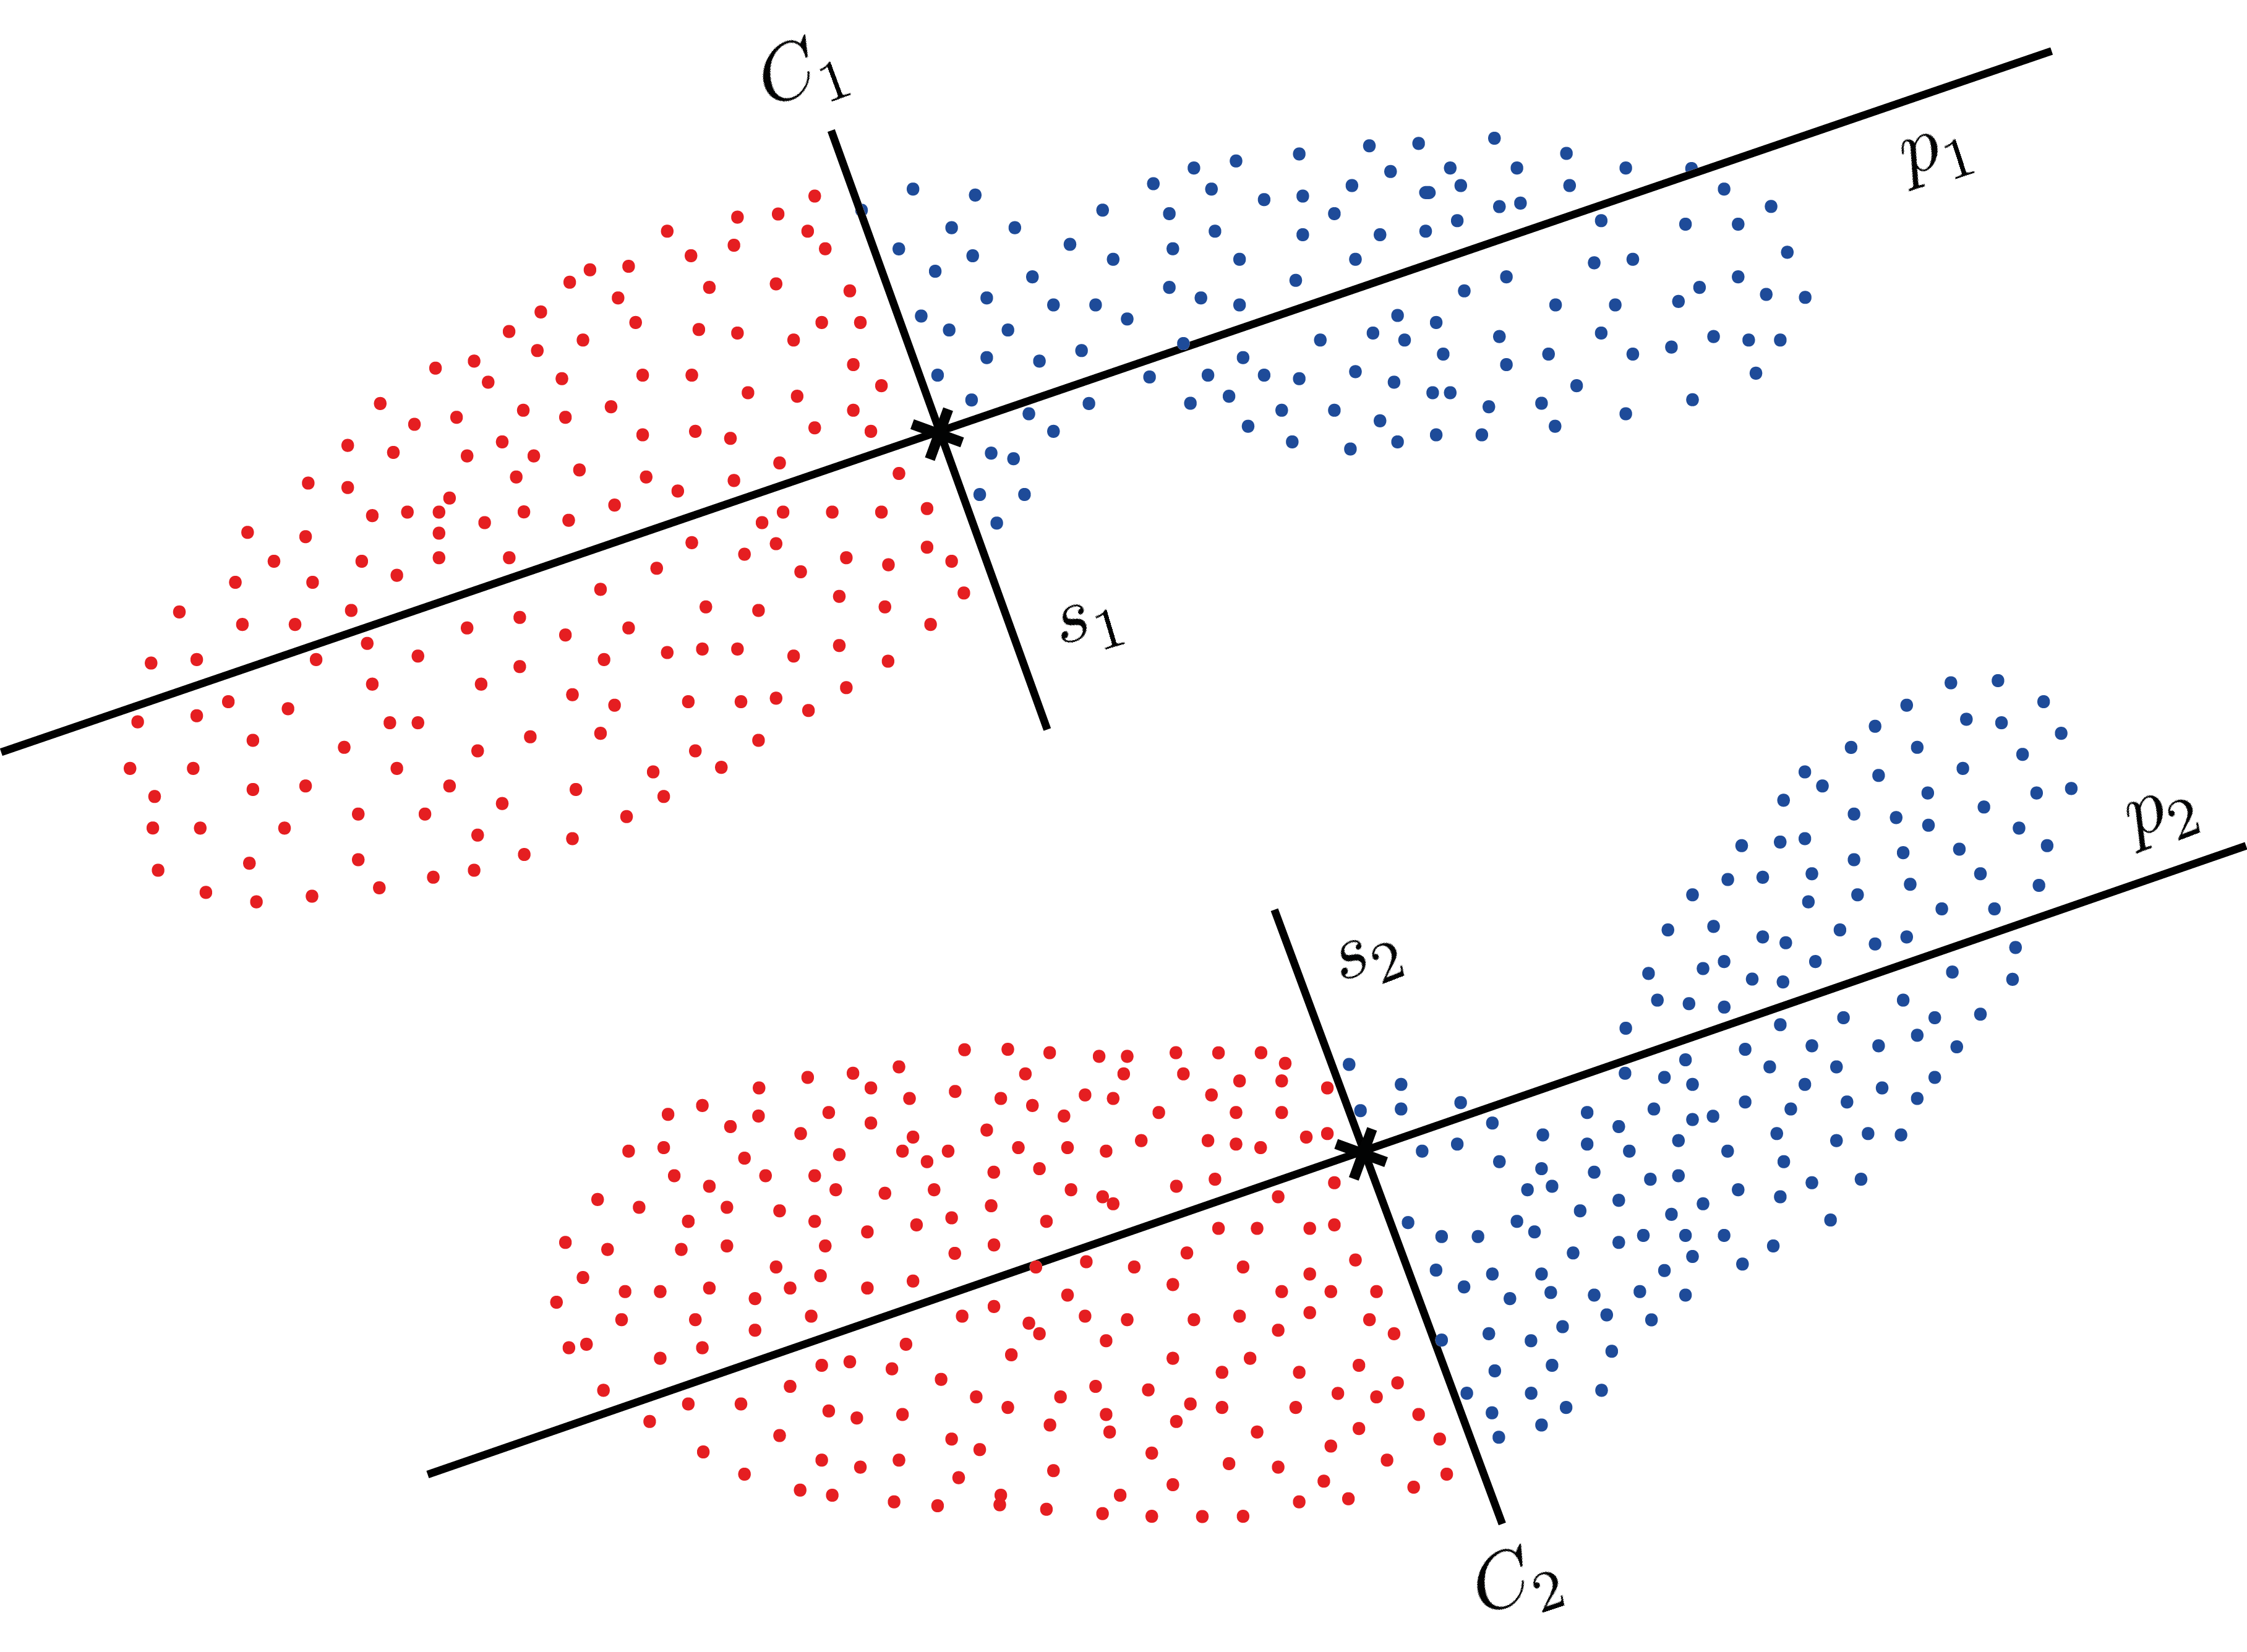
\includegraphics[width=0.7\linewidth]{illustration_axes}
 	\caption{Dividing \textit{S\textsubscript{0}} and \textit{D\textsubscript{0}} into clusters by the divider \textit{d} to match them with ICP.}
 	\label{fig:dc_axes_2p}
 \end{figure}

 \begin{figure}
 	\centering
 	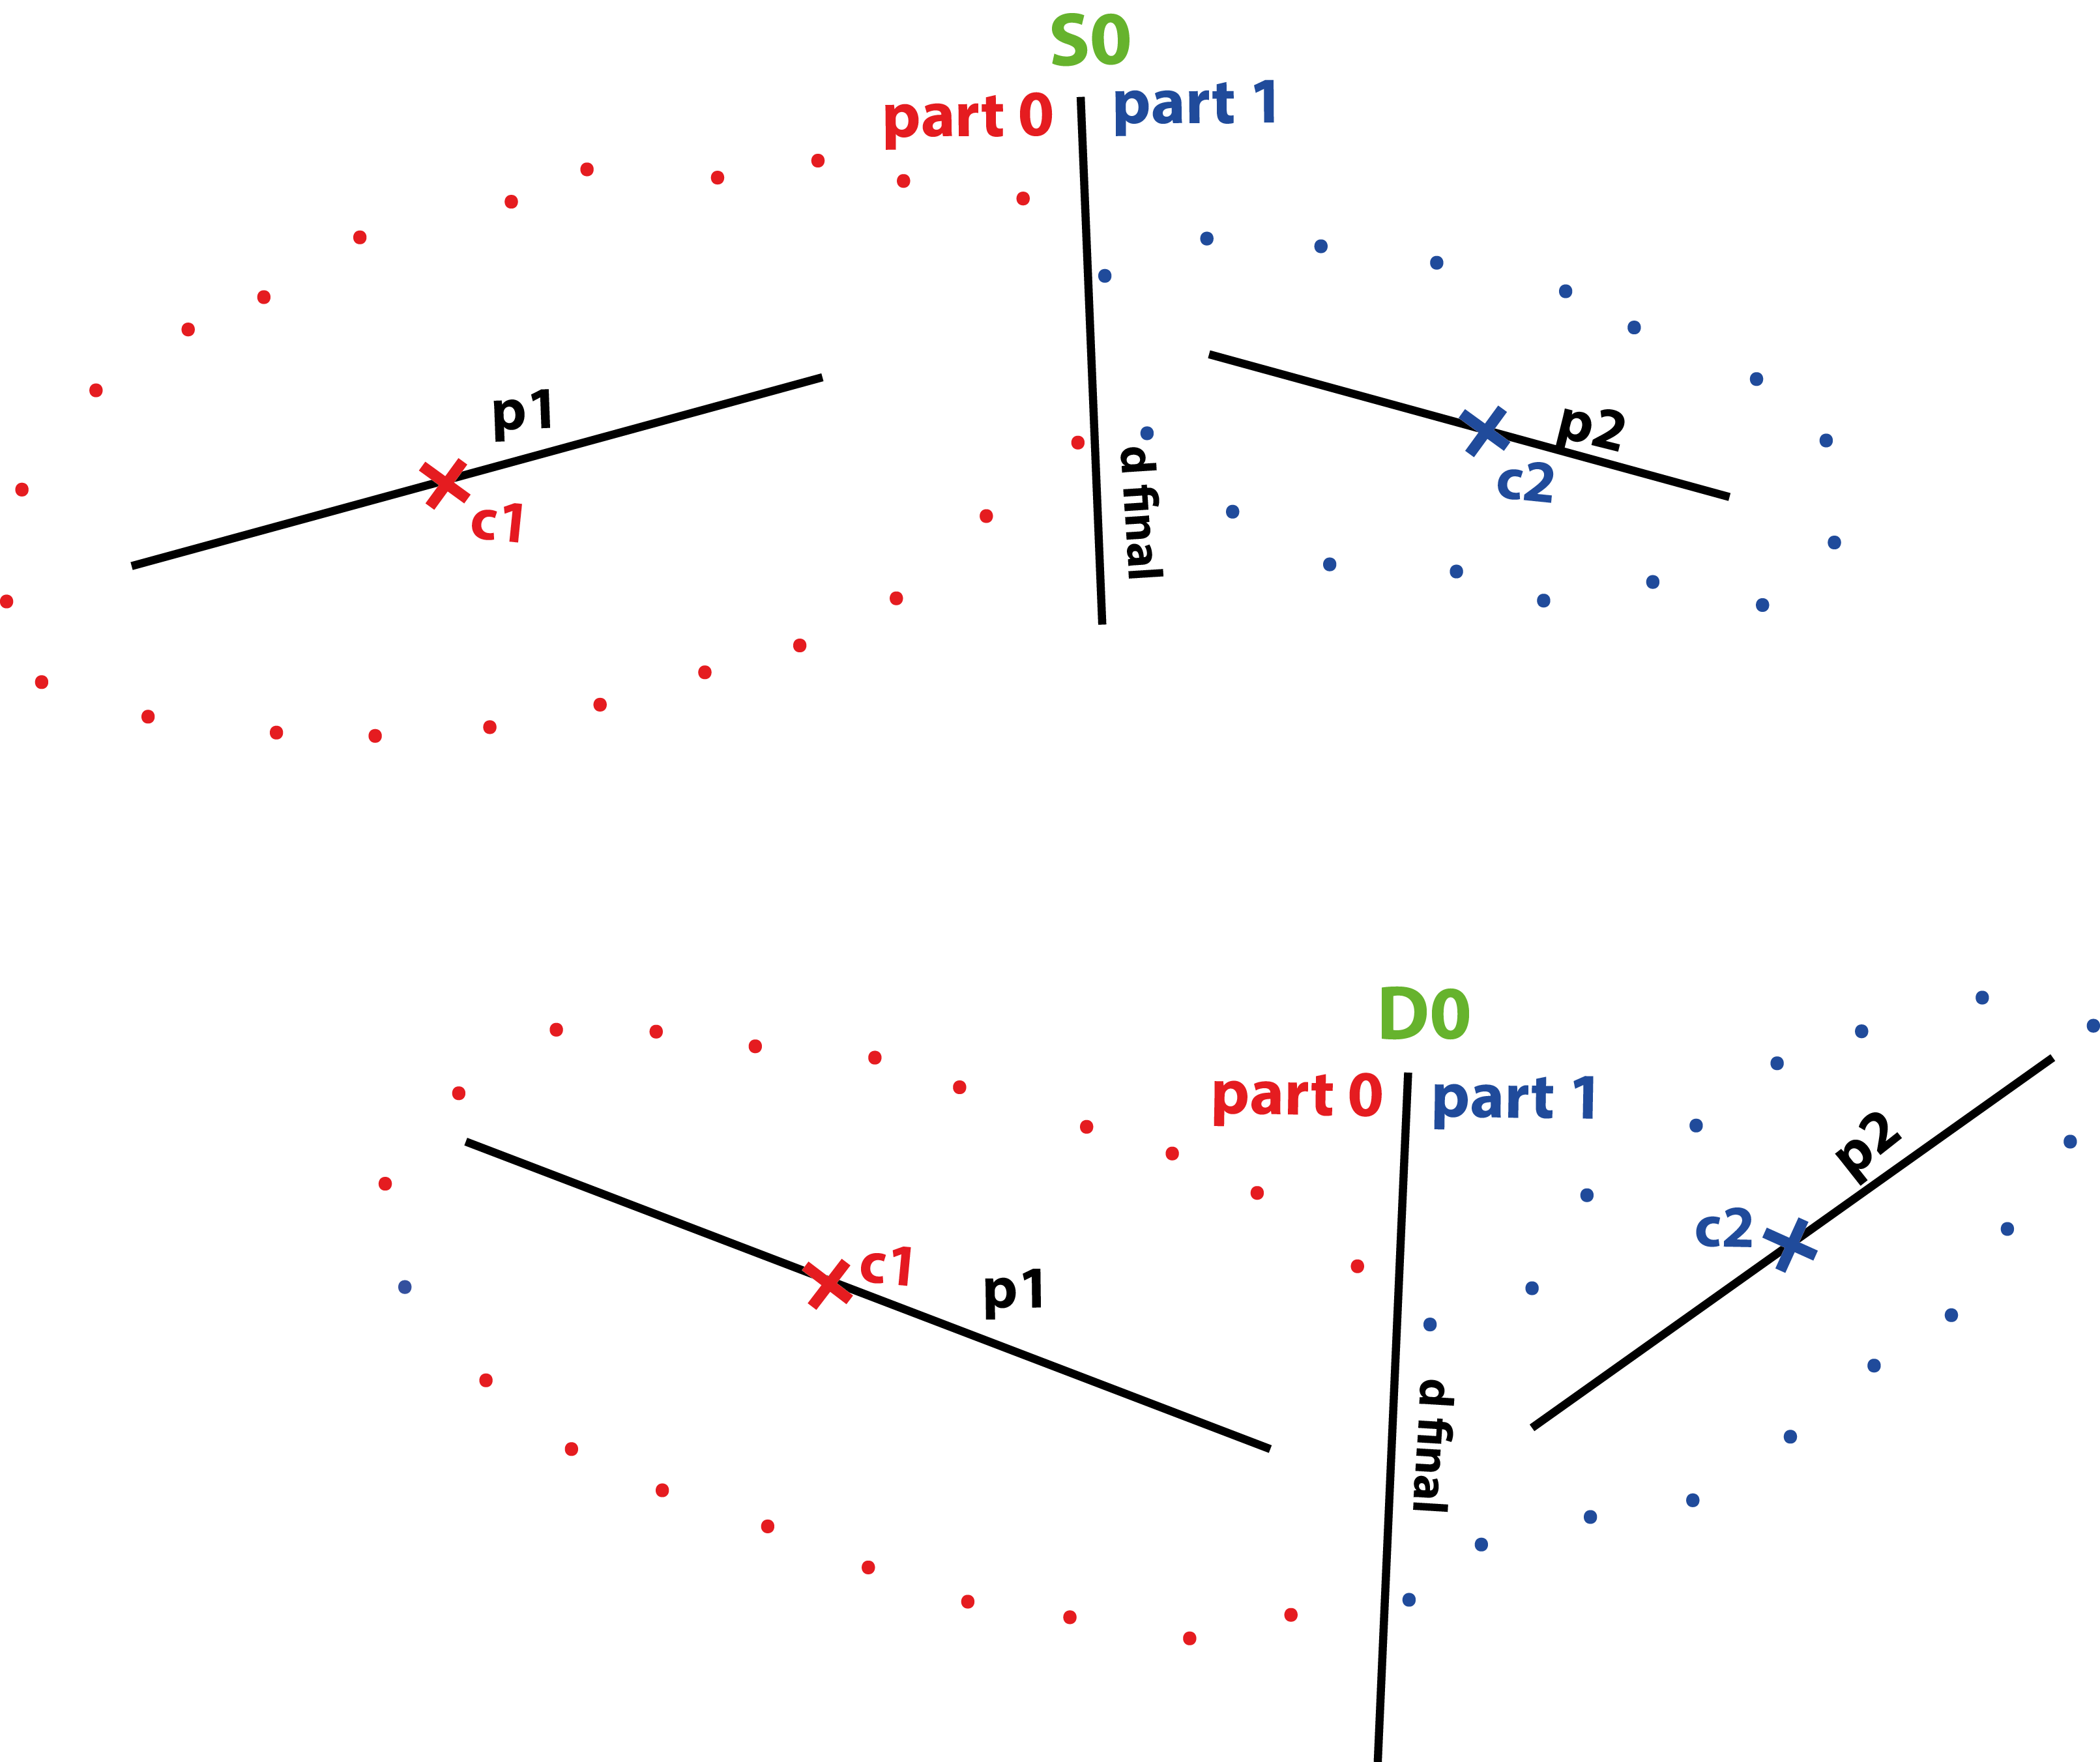
\includegraphics[width=0.7\linewidth]{illustration_results}
 	\caption{Assigning of the rigid parts \textit{P =(part\textsubscript{0}, part\textsubscript{1})} after termination of segmentation process.}
 	\label{fig:dc_results_2p}
 \end{figure}
 
 \subsection{Implementation Steps}
 
 \begin{enumerate}
 	\item The centroids \textit{c\textsubscript{S}} and \textit{c\textsubscript{D}} of \textit{S\textsubscript{0}} and \textit{D\textsubscript{0}} are computed.
 	
 	\item The principal axis \textit{p\textsubscript{S}} and \textit{p\textsubscript{D}}  are computed through \textit{c\textsubscript{S}} and \textit{c\textsubscript{D}} in order to orient the point clouds horizonally around their centroids.
 	
 	\item The secondary axis \textit{s\textsubscript{S}} and \textit{s\textsubscript{D}} perpendicular to \textit{p\textsubscript{S}} and \textit{p\textsubscript{D}} through \textit{c\textsubscript{S}} and \textit{c\textsubscript{D}} are computed.
 	
 	\item The dividers \textit{d\textsubscript{S}} and \textit{d\textsubscript{T}} to segment \textit{S\textsubscript{0}} and \textit{D\textsubscript{0}} into its assumed two rigid parts are initialized with the secondary axis \textit{s\textsubscript{S}} and \textit{s\textsubscript{D}}.
 	
 	\item The points \textit{P\textsubscript{0...N}} of \textit{S\textsubscript{0}}  are either allocated to \textit{S\textsubscript{left}} or \textit{S\textsubscript{right}} depending on its position to \textit{d\textsubscript{S}}. The same procedure is done with all points of \textit{D\textsubscript{0}}.
 	
 	\item ICP is computed between the rigid parts \textit{S\textsubscript{left}} and \textit{D\textsubscript{left}} as well as \textit{S\textsubscript{right}} and \textit{D\textsubscript{right}}.
 	
 	\item An error distance \textit{e\textsubscript{left}} and \textit{e\textsubscript{right}} is obtained. The part with the most error per point is assumed to be not rigid which gives back an indicator where to divide \textit{S\textsubscript{0}} and \textit{D\textsubscript{0}}.
 	
 	\item The dividers \textit{d\textsubscript{S}} and \textit{d\textsubscript{D}} are shifted to the direction of the highest error. To be continued from step 5 until the total error \textit{e\textsubscript{total}} doesn't get smaller.
 \end{enumerate}

\subsection{Results}

Results from easy examples. Not working for human, as by dividing of one cluster, breaking down into single clusters (see Figure X). Another approach, e.g. using LRP as an initial alignment to then recursively segment the clusters linked to the LRP. Clusters not matching, as they don't have the same number of points, each point can only have one neighboring point. Or dividing clusters that they all have the same amount of points. In case of a more complex object where one rigid part can be linked with a high number of rigid parts (upper body of a humen) another approach has to be found, as the skeleton structure is different than from a chain. (see Figure \ref{fig:dc_results_2p}).

\subsection{Possible Improvements}

\subsubsection{Same amount of points of associated clusters}

\subsubsection{Check clusters after subdividing}

After subdividing, only two clusters should come up.

\subsubsection{LRP as initial alignment}

As only objects with rigid parts arranged like a chain are possible with this approach, another improvement/algorithm has to be pursued (see section \ref{sec:LRP}).

\section{LRP as initial alignment}
\label{sec:LRP}

Instead of cutting the object initially in half, as an initial step the largest rigid part is found and recursively from there all other linked parts can be detected.

\subsection{Overview}
As an initial step, the LRP algorithm tries to find the most reliable correspondences, the so-called largest rigid part (LRP), subsequently all other parts are detected that are linked to the LRP. The initial alignment stage tries to find sparse correspondences between two point clouds by applying a single rigid transformation to detect the largest subsets of points in two point clouds. Starting from the LRP all other parts are detected recursively.

\subsection{Algorithm} 

\subsubsection{Finding the LRP}

The algorithm also takes two point clouds \textit{S\textsubscript{0}} and \textit{T\textsubscript{0}} of the same object in different configurations as input.
The goal is to find a single rigid transformation \textit{T\textsubscript{init}} for all points of \textit{S\textsubscript{0}} to get potential corresponding points \textit{C\textsubscript{0} = \{(s\textsubscript{i}, t\textsubscript{j})\}} in \textit{T\textsubscript{0}}. For that, local descriptors of \textit{S\textsubscript{0}} and \textit{T\textsubscript{0}} are computed. The requirement for a sparse correspondance between two points \textit{s\textsubscript{i}} and \textit{t\textsubscript{j}}  is that they are \textit{reciprocal}, which means that the Euclidean distance \textit{d(s\textsubscript{i}, t\textsubscript{j})} between them is the smallest in both directions. Some of the sparse correspondances are asumed to be wrong. Therefore, RANSAC is used on the sparse correspondances \textit{C\textsubscript{0}} to estimate a rigid alignment that is supported by the largest number of points \textit{n} from \textit{S\textsubscript{0}} and \textit{T\textsubscript{0}}. To assign the LRP in \textit{S\textsubscript{0}} and \textit{T\textsubscript{0}}, the biggest point clusters \textit{C\textsubscript{s}} and \textit{C\textsubscript{t}} of the overlapping area \textit{G\textsubscript{s} = \{C\textsubscript{1}, ... , C\textsubscript{n}\} } and \textit{G\textsubscript{t} = \{C\textsubscript{1}, ... , C\textsubscript{n}\} } are detected. 


\subsubsection{Part discovery}

The remaining clusters from \textit{S\textsubscript{0}} and \textit{T\textsubscript{0}} that have not been registered yet are matched recursively by starting with clusters connected to already matched parts. First, all matched parts are excluded from the input point clouds  \textit{G\textsubscript{s(l+1)}} = \textit{S\textsubscript{0}} - \textit{C\textsubscript{sl}} and \textit{G\textsubscript{t(l+1)}} = \textit{T\textsubscript{0}} - \textit{C\textsubscript{tl}} defining \textit{l} as the number of already matched parts \{1, ..., n\}, \textit{C\textsubscript{sl}}. For that clusters are formed, using region taking into account that they are attached to already registered parts. The algorithm explained is applied until all body parts have been discovered.

\subsection{Steps}

\begin{enumerate}
	\item The centroids \textit{c\textsubscript{s}} and \textit{c\textsubscript{t}} of \textit{S\textsubscript{0}} and \textit{T\textsubscript{0}} are computed.
	
	\item The principal axis \textit{p\textsubscript{s}} and \textit{p\textsubscript{t}}  are computed through \textit{c\textsubscript{s}} and \textit{c\textsubscript{t}} in order to horizontally orient the objects around their centroids.
	
	\item The ICP is conducted as a first guess to find a transformation \textit{T\textsubscript{init}} for all points from \textit{S\textsubscript{0}} that results in the highest number of corresponding points \textit{n} in \textit{T\textsubscript{0}}, given the threshold \textit{T}.
	
	\item \textit{C\textsubscript{0}} contains the corresponding points from S\textsubscript{0} and T\textsubscript{0}, resulting from \textit{T\textsubscript{init}(S\textsubscript{0})}.
	
	\item The RANSAC approach is applied on \textit{C\textsubscript{0}} to find a  \textit{T\textsubscript{f}} that results in the highest number of corresponding points \textit{n} between \textit{T\textsubscript{f}(S\textsubscript{0})} and \textit{T\textsubscript{0}}.
	
	\item The LRP is assigned to \textit{C\textsubscript{s}} and \textit{C\textsubscript{t}} from the resulting point clusters \textit{G\textsubscript{s}} and \textit{G\textsubscript{t}}.
	
	\item Starting from parts that are connected to the LRP, corresponding points \textit{C\textsubscript{i}} for unmatched points from \textit{S\textsubscript{0}} and \textit{T\textsubscript{0}} are seeked. The clusters are given as a input from Step 5. 
		
\end{enumerate}

\section{Other approaches}

\subsection{Points-to-Ellipse fitting}

\subsection{Algorithm}

This algorithm only requires one point cloud containing \textit{m} points \{\textit{pt\textsubscript{0}, ..., pt\textsubscript{m}}\}. The basic idea is to segment the non-rigid object  \textit{S\textsubscript{0}} into its rigid parts \textit{part\textsubscript{1}} and {part\textsubscript{2}} by fitting ellipses to its rigid parts. 
\textit{S\textsubscript{0}} is divided perpendicular to its principal axis \textit{p\textsubscript{0}} into two assumed rigid parts \textit{S\textsubscript{left}} and \textit{S\textsubscript{right}}, initially defining the divider \textit{d} with the secondary axis \textit{s\textsubscript{0}}. The points of \textit{S\textsubscript{left}} and \textit{S\textsubscript{right}} are verified to 
form an ellipse by using its formular

\begin{equation}
\dfrac{x^2}{r_1^2} + \dfrac{y^2}{r_2^2} = 1
\end{equation}

Assuming to verify \textit{S\textsubscript{left}} forming an ellipse, \textit{r\textsubscript{1}} is half the length of the principal axis \textit{p\textsubscript{left}} of \textit{S\textsubscript{left}} through its centroid \textit{c\textsubscript{left}}. Furthermore, \textit{r\textsubscript{2}} is half the length of the secondary axis {s\textsubscript{left}} of \textit{S\textsubscript{left}}. Thereby, the centroid \textit{c\textsubscript{left}} needs to be located in the origin (0,0). 
Now, to check whether a point \textit{pt\textsubscript{i}} of \textit{S\textsubscript{left}} is located on the ellipse, the formular is remodeled and its x values is applied. 

\begin{equation}
(1 -  \dfrac{x^2}{r_1^2}) \cdot {r_2^2} = y^2
\end{equation}

The resulting y-value of the ellipse is compared to the points actual y-value. Given a certain threshold $\tau$ a point either accounts to the number of total points lying on the ellipse \textit{n}, or not.

\begin{equation}
n = \sum_{i=0}^{m}\begin{cases}1 \quad if \quad \|pt_i.y^2 - y^2 \| < \tau \\ 0 \quad otherwise\end{cases}
\end{equation}

The algorithm is repeated by sliding \textit{d} in the direction of the highest error \textit{e}. To be continued until the total error \textit{e\textsubscript{total} = e\textsubscript{left} + \textsubscript{right}} reaches its minimum.

\subsection{Steps}

\begin{enumerate}
	\item The centroid \textit{c\textsubscript{0}}  of \textit{S\textsubscript{0}} is computed.
	
	\item The principal axis \textit{p\textsubscript{0}} is computed through \textit{c\textsubscript{0}} and \textit{S\textsubscript{0}} horizontally oriented. 
	
	\item The secondary axis \textit{s\textsubscript{0}}  perpendicular to \textit{p\textsubscript{0}} through \textit{c\textsubscript{0}} is computed.
	
	\item The divider \textit{d} is initialized with the secondary axis \textit{s\textsubscript{0}} to segment \textit{S\textsubscript{0}} into two assumed rigid parts .
	
	\item The points of \textit{S\textsubscript{0}} are either allocated to \textit{S\textsubscript{left}} or \textit{S\textsubscript{right}} depending on its position to \textit{d\textsubscript{0}}.
	
	\item The ellipse formular is applied on \textit{S\textsubscript{left}} and \textit{S\textsubscript{right}}.
	
	\item An error \textit{e\textsubscript{left}} and \textit{e\textsubscript{right}} is obtained implying how many points of \textit{S\textsubscript{left}} and \textit{S\textsubscript{right}} form an ellipse. 
	
	\item The divider \textit{d} is shifted to the direction of the highest error. To be continued from step 5 until the total error \textit{e\textsubscript{total}} doesn't get smaller. 
\end{enumerate}

\subsection{Results}

\subsection{Reusing detected shapes}

After termination of the algorithm, one point cloud can be segmented into its rigid parts P \{part\textsubscript{1}, ..., part\textsubscript{n}\}. Their variables like the ellipses' centroid \textit{c\textsubscript{i}} and radii \textit{r\textsubscript{1}}, \textit{r\textsubscript{2}} can be used to segment similar point clouds in different configurations. As the shapes to be matched are already known, e.g. how they are linked, finding the position to be segmented is a lot easier.



\section{General Results}

\section{Improvements}

\section{Future work}

The approaches implemented in 2D are then implemented in 3D using the PCL. 

